\documentclass{article}
\usepackage{hyperref}
\usepackage{graphicx}
\usepackage{float}
\usepackage{amsmath}

\title{Computer Vision HW9 Report}
\author{B01902044 Steven Lin}
\date{2015-12-10}

\newcommand{\code}[1]{\texttt{#1}}

\begin{document}

\pagenumbering{gobble}
\maketitle
\newpage

\pagenumbering{arabic}

\tableofcontents
\newpage

% ---------- 1st section: source code ---------- %
\section{Source Code}
This part of the report will go through some important snippets of my source code. For source code file, please check out the \code{hw9.py} file in the directory submitted.

\subsection{Principle Code Sneak Peek}
First, we will take a look at the overall structure of my code. And furthermore we will have some brief explanation for the implementation of the 7 operators in this homework.

\subsubsection{Functions Overview}
In this homework, we are asked to implement 7 different kinds of edge detection methods. And for every method, I created a function for it. \\
The following snapshot shows a list of 7 functions corresponding to one of the detection methods respectively. \\
\begin{figure}[H]
  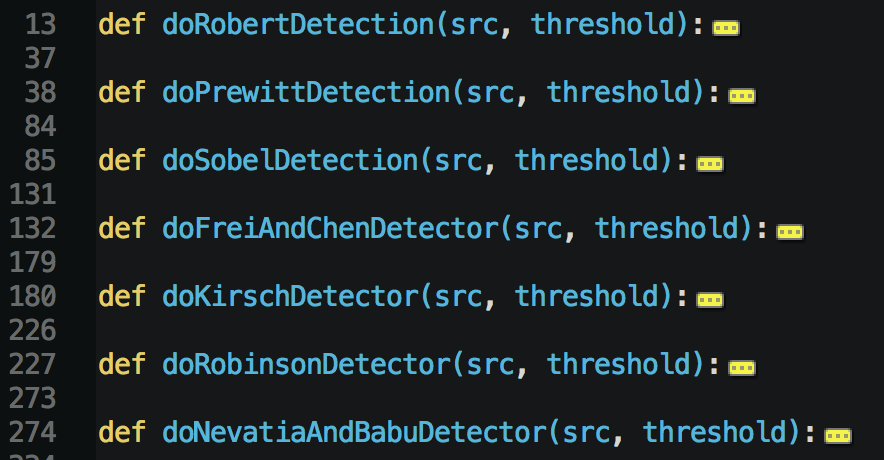
\includegraphics[width=\linewidth]{img/functions_overview.png}
  \caption{Essential Functions Overview}
  \label{fig:functions_overview}
\end{figure}
All of the functions above take 2 parameters: \code{src} and \code{threshold}. For more information about these two required parameters, please see to the description in the following list.
\begin{description}
  \item[\code{src}] \hfill \\
  The source image for the functions to detect edges.
  \item[\code{threshold}] \hfill \\
  The threshold for the operator with regard to the specific edge detection method.
\end{description}

\subsubsection{Common Gradient Magnitude}
The most common type of edge detection process uses a gradient operator which calculate the gradient magnitude \code{g(x, y)} from the intensity values of neighboring pixels. Mathematically, it is computed this way:
$$ g(x, y) \cong (\Delta x^{2} + \Delta y^{2})^{\frac{1}{2}} $$
and the gradient direction would thus be:
$$ \theta(x, y) \cong atan(\frac{\Delta y}{\Delta x}) $$
\paragraph{Detection methods of this type}
Robert's, Prewitt's, Sobel's, Frei and Chen's. \\

For this type of operators, I first created two empty 2D matrices with each of them representing $ \Delta x $ and $ \Delta y $, and after the completion of computing both of the matrices, I utilize the code fragment as in the figure below to determine the final gradient value.
\begin{figure}[H]
  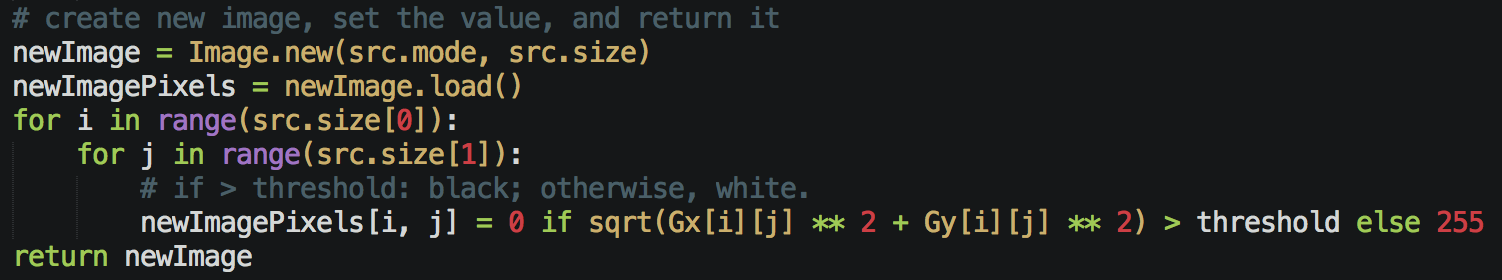
\includegraphics[width=\linewidth]{img/normal_gradient.png}
  \caption{Common Gradient Calculation}
  \label{fig:normal_gradient}
\end{figure}

\subsubsection{Maximum Magnitude Type}
The other type of magnitude calculation involves multiple (usually greater than two) masks. With convolving every one of the masks respectively, we determine the final gradient value \code{g(x, y)} by this formula:
$$ g(x, y) = \max_{i=1..N}(convolved\_value(mask_{i})) $$
where \code{N} is the number of masks defined/used this operator. \\
\paragraph{Detection methods of this type}
Kirsch's, Robinson's, Nevatia-Babu 5x5 Operator. \\

As for this type of operators, when calculating \code{g(x, y)} for every pixel on the source image, I first retrieve the intensity values of its neighbors that are required according to the definition of the operator. I will then have two \code{list} (i.e., array), one for intensity values needed, and the other for coefficient defined by the operator. The gradient value will therefore be computed this way:
\begin{align*}
g(x, y) &= \max_{i=1..N}(compasses_{i}) \\
compasses_{i} &= coeff_{i} \cdot neighbors
\end{align*}
where \code{N} is the number of masks (i.e., compasses), \code{coeff} is the coefficient array, \code{neighbors} is the array storing intensity values of neighbors needed. The actual implementation of these equations are as shown in the following code snippet.
\begin{figure}[H]
  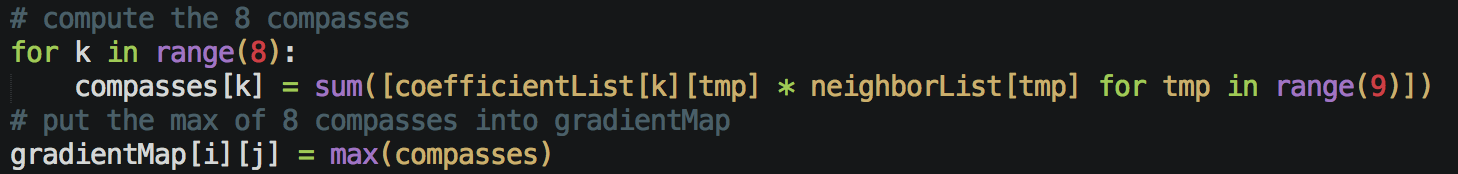
\includegraphics[width=\linewidth]{img/max_gradient.png}
  \caption{Max Gradient Calculation}
  \label{fig:max_gradient}
\end{figure}

\subsection{Parameters (Threshold)}
\begin{description}
  \item[Robert's Operator] \hfill \\
  my threshold = 30
  \item[Prewitt's Edge Detector] \hfill \\
  my threshold = 24
  \item[Sobel's Edge Detector] \hfill \\
  my threshold = 38
  \item[Frei and Chen's Gradient Operator] \hfill \\
  my threshold = 30
  \item[Kirsch's Compass Operator] \hfill \\
  my threshold = 135
  \item[Robinson's Compass Operator] \hfill \\
  my threshold = 43
  \item[Nevatia-Babu 5x5 Operator] \hfill \\
  my threshold = 12500
\end{description}

% ---------- 2nd section: results ---------- %
\section{Results}
All the resulted images are properly saved and submitted along with this report document. You may go check them out if you'd like to.

\subsection{Robert's Operator}
\begin{figure}[H]
  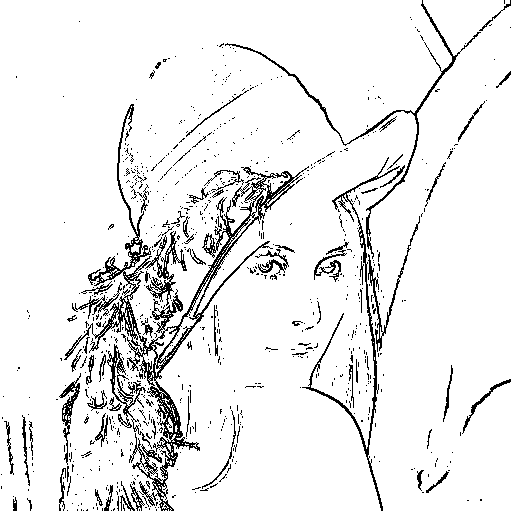
\includegraphics[width=\linewidth]{img/robert_30.png}
  \caption{Robert's with threshold=30}
  \label{fig:robert_30}
\end{figure}

\subsection{Prewitt's Edge Detector}
\begin{figure}[H]
  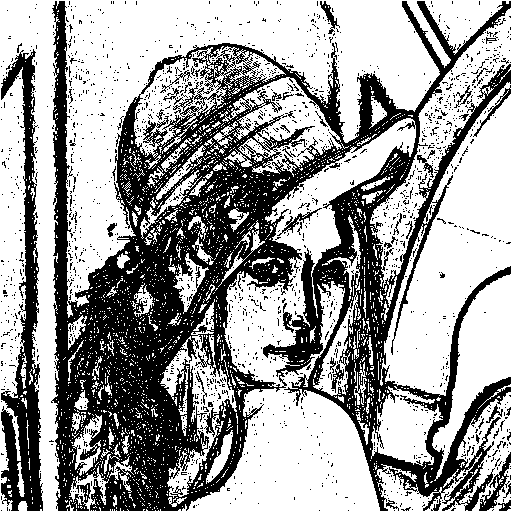
\includegraphics[width=\linewidth]{img/prewitt_24.png}
  \caption{Prewitt's with threshold=24}
  \label{fig:prewitt_24}
\end{figure}

\subsection{Sobel's Edge Detector}
\begin{figure}[H]
  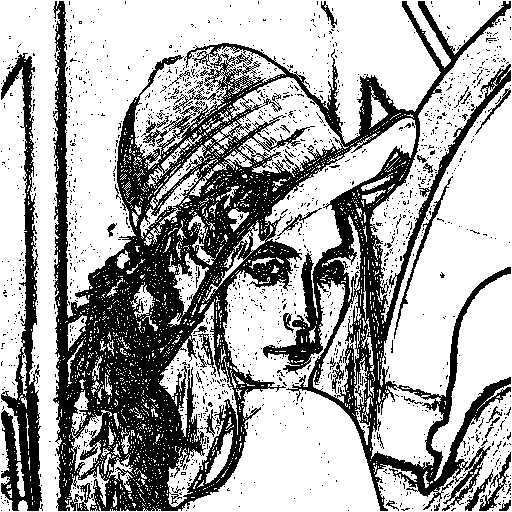
\includegraphics[width=\linewidth]{img/sobel_38.png}
  \caption{Sobel's with threshold=38}
  \label{fig:sobel_38}
\end{figure}

\subsection{Frei and Chen's Gradient Operator}
\begin{figure}[H]
  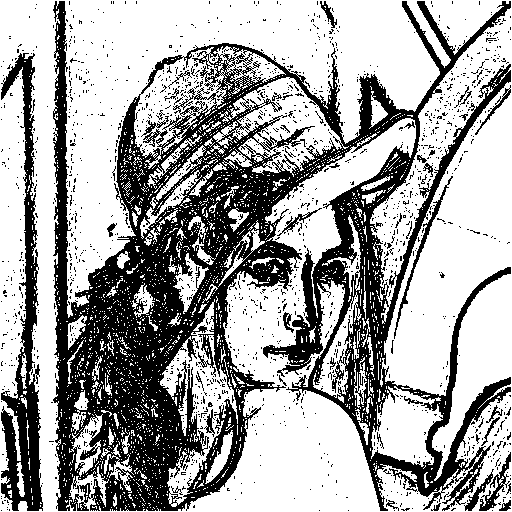
\includegraphics[width=\linewidth]{img/frei_and_chen_30.png}
  \caption{Frei and Chen's with threshold=30}
  \label{fig:frei_and_chen_30}
\end{figure}

\subsection{Kirsch's Compass Operator}
\begin{figure}[H]
  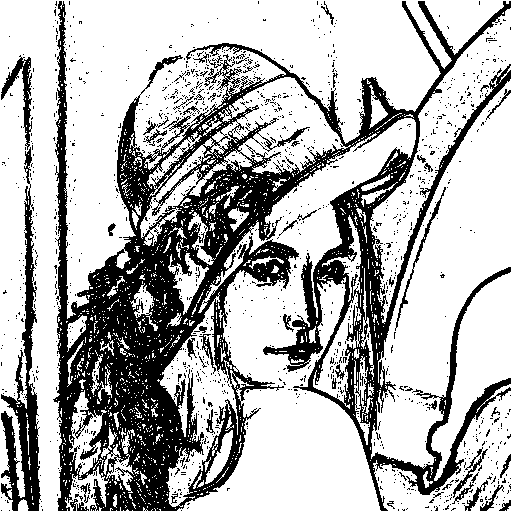
\includegraphics[width=\linewidth]{img/kirsch_135.png}
  \caption{Kirsch's with threshold=135}
  \label{fig:kirsch_135}
\end{figure}

\subsection{Robinson's Compass Operator}
\begin{figure}[H]
  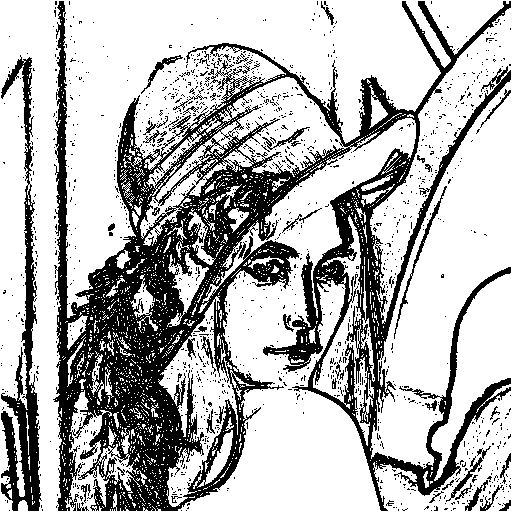
\includegraphics[width=\linewidth]{img/robinson_43.png}
  \caption{Robison's with threshold=43}
  \label{fig:robinson_43}
\end{figure}

\subsection{Nevatia-Babu 5x5 Operator}
\begin{figure}[H]
  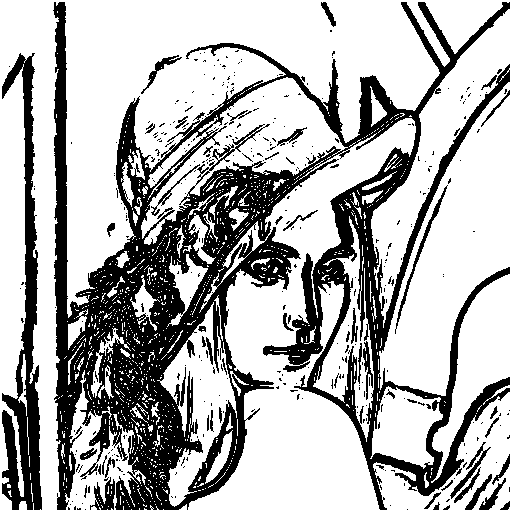
\includegraphics[width=\linewidth]{img/nevatia_and_babu_12500.png}
  \caption{Nevatia-Babu's with threshold=12500}
  \label{fig:nevatia_and_babu_12500}
\end{figure}

\end{document}